\documentclass{beamer}


%\usepackage{listings}      % Activate for custom appearance.  Other themes can be found online.  Search ``beamer themes''
\usepackage{listings}  
\usepackage{graphicx}
\usetheme{Darmstadt}
\usecolortheme{dolphin}
\def \tbs {\textbackslash}
\input xy
\xyoption{all}
\title{Monotone Catenary Degree \newline in Numerical Monoids}
\author{D. Gonzalez, C. Wright, J. Zomback}
\date{August 4, 2015}

\begin{document}

\newtheorem{conjecture}{Conjecture}
\newtheorem{proposition}{Proposition}
\frame{\titlepage}

%%%%%%%%%%%%%%%%%%%%%%%%%%%%%%%%%%%%
\section[Introduction]{Introduction}

\frame{\frametitle{Outline}
\pause
\begin{itemize}
	\item Definitions \pause
	\item Arithmetic Monoids \pause
	\item Generalized Arithmetic Monoids \pause
	\item Difference between Monotone and Regular Catenary Degree \pause
\end{itemize}

}

\frame{\frametitle{Construction of a Catenary Graph}

\begin{minipage}[t]{0.48\linewidth}
\xymatrix{
	&&{\bullet} \ar@{-}[d]_3 \ar@{-}[dr]^>>>>4 \ar@/^1pc/@{-}[drr]^>>>3 \\
	&&{\bullet} \ar@{-}[r]^<<<<1 \ar@{-}[d]_2 \ar@{-}[dr]|5 & {\bullet} \ar@{-}[d]^3 \ar@{-}[dl]|5 & {\bullet} \ar@{-}[l]_>>>>1 \\
	&&{\bullet} \ar@/^2pc/@{-}[uu]^2 \ar@{-}[r]_<<<<2 \ar@{-}[d]_2 & {\bullet} \ar@/^/@{-}[dl]^<<<<2 \ar@/_/@{-}[ur]_>>>>3 \\
	&&{\bullet} \ar@/^2pc/@{-}[uu]^2
} \pause
\end{minipage}
\begin{minipage}[t]{0.48\linewidth}
\begin{itemize}

	\item Remove edges with the largest distances \pause
	\item Continue until disconnected \pause
	\item Final distance removed is catenary degree

\end{itemize}
$$\phantom{c(m)=3}$$
\end{minipage}

}

\frame{\frametitle{Construction of a Catenary Graph}

\begin{minipage}[t]{0.48\linewidth}
\xymatrix{
	&&{\bullet} \ar@{-}[d]_3 \ar@{-}[dr]^>>>>4 \ar@/^1pc/@{-}[drr]^>>>3 \\
	&&{\bullet} \ar@{-}[r]^<<<<1 \ar@{-}[d]_2 \ar@{-}[dr]|{\mathbf{5}} & {\bullet} \ar@{-}[d]^3 \ar@{-}[dl]|{\mathbf{5}} & {\bullet} \ar@{-}[l]_>>>>1 \\
	&&{\bullet} \ar@/^2pc/@{-}[uu]^2 \ar@{-}[r]_<<<<2 \ar@{-}[d]_2 & {\bullet} \ar@/^/@{-}[dl]^<<<<2 \ar@/_/@{-}[ur]_>>>>3 \\
	&&{\bullet} \ar@/^2pc/@{-}[uu]^2
}
\end{minipage}
\begin{minipage}[t]{0.48\linewidth}
\begin{itemize}

	\item Remove edges with the largest distances 
	\item Continue until disconnected 
	\item Final distance removed is catenary degree

\end{itemize}
$$\phantom{c(m)=3}$$
\end{minipage}

}

\frame{\frametitle{Construction of a Catenary Graph}

\begin{minipage}[t]{0.48\linewidth}
\xymatrix{
	&&{\bullet} \ar@{-}[d]_3 \ar@{-}[dr]^>>>>4 \ar@/^1pc/@{-}[drr]^>>>3 \\
	&&{\bullet} \ar@{-}[r]^<<<<1 \ar@{-}[d]_2 \ar@{.}[dr] & {\bullet} \ar@{-}[d]^3 \ar@{.}[dl] & {\bullet} \ar@{-}[l]_>>>>1 \\
	&&{\bullet} \ar@/^2pc/@{-}[uu]^2 \ar@{-}[r]_<<<<2 \ar@{-}[d]_2 & {\bullet} \ar@/^/@{-}[dl]^<<<<2 \ar@/_/@{-}[ur]_>>>>3 \\
	&&{\bullet} \ar@/^2pc/@{-}[uu]^2
}
\end{minipage}
\begin{minipage}[t]{0.48\linewidth}
\begin{itemize}

	\item Remove edges with the largest distances 
	\item Continue until disconnected 
	\item Final distance removed is catenary degree

\end{itemize}
$$\phantom{c(m)=3}$$
\end{minipage}

}

\frame{\frametitle{Construction of a Catenary Graph}

\begin{minipage}[t]{0.48\linewidth}
\xymatrix{
	&&{\bullet} \ar@{-}[d]_3 \ar@{-}[dr]^>>>>{\mathbf{4}} \ar@/^1pc/@{-}[drr]^>>>3 \\
	&&{\bullet} \ar@{-}[r]^<<<<1 \ar@{-}[d]_2 \ar@{.}[dr] & {\bullet} \ar@{-}[d]^3 \ar@{.}[dl] & {\bullet} \ar@{-}[l]_>>>>1 \\
	&&{\bullet} \ar@/^2pc/@{-}[uu]^2 \ar@{-}[r]_<<<<2 \ar@{-}[d]_2 & {\bullet} \ar@/^/@{-}[dl]^<<<<2 \ar@/_/@{-}[ur]_>>>>3 \\
	&&{\bullet} \ar@/^2pc/@{-}[uu]^2
}
\end{minipage}
\begin{minipage}[t]{0.48\linewidth}
\begin{itemize}

	\item Remove edges with the largest distances 
	\item Continue until disconnected 
	\item Final distance removed is catenary degree

\end{itemize}
$$\phantom{c(m)=3}$$
\end{minipage}

}

\frame{\frametitle{Construction of a Catenary Graph}

\begin{minipage}[t]{0.48\linewidth}
\xymatrix{
	&&{\bullet} \ar@{-}[d]_3 \ar@{.}[dr]^>>>>{\phantom{\mathbf{4}}} \ar@/^1pc/@{-}[drr]^>>>3 \\
	&&{\bullet} \ar@{-}[r]^<<<<1 \ar@{-}[d]_2 \ar@{.}[dr] & {\bullet} \ar@{-}[d]^3 \ar@{.}[dl] & {\bullet} \ar@{-}[l]_>>>>1 \\
	&&{\bullet} \ar@/^2pc/@{-}[uu]^2 \ar@{-}[r]_<<<<2 \ar@{-}[d]_2 & {\bullet} \ar@/^/@{-}[dl]^<<<<2 \ar@/_/@{-}[ur]_>>>>3 \\
	&&{\bullet} \ar@/^2pc/@{-}[uu]^2
}
\end{minipage}
\begin{minipage}[t]{0.48\linewidth}
\begin{itemize}

	\item Remove edges with the largest distances 
	\item Continue until disconnected 
	\item Final distance removed is catenary degree

\end{itemize}
$$\phantom{c(m)=3}$$
\end{minipage}

}

\frame{\frametitle{Construction of a Catenary Graph}

\begin{minipage}[t]{0.48\linewidth}
\xymatrix{
	&&{\bullet} \ar@{-}[d]_{\mathbf{3}} \ar@{.}[dr]^>>>>{\phantom{\mathbf{4}}} \ar@/^1pc/@{-}[drr]^>>>{\mathbf{3}} \\
	&&{\bullet} \ar@{-}[r]^<<<<1 \ar@{-}[d]_2 \ar@{.}[dr] & {\bullet} \ar@{-}[d]^{\mathbf{3}} \ar@{.}[dl] & {\bullet} \ar@{-}[l]_>>>>1 \\
	&&{\bullet} \ar@/^2pc/@{-}[uu]^2 \ar@{-}[r]_<<<<2 \ar@{-}[d]_2 & {\bullet} \ar@/^/@{-}[dl]^<<<<2 \ar@/_/@{-}[ur]_>>>>{\mathbf{3}} \\
	&&{\bullet} \ar@/^2pc/@{-}[uu]^2
}
\end{minipage}
\begin{minipage}[t]{0.48\linewidth}
\begin{itemize}

	\item Remove edges with the largest distances 
	\item Continue until disconnected 
	\item Final distance removed is catenary degree

\end{itemize}
$$\phantom{c(m)=3}$$
\end{minipage}

}

\frame{\frametitle{Construction of a Catenary Graph}

\begin{minipage}[t]{0.48\linewidth}
\xymatrix{
	&&{\bullet} \ar@{.}[d]_{\phantom{\mathbf{3}}} \ar@{.}[dr]^>>>>{\phantom{\mathbf{4}}} \ar@/^1pc/@{.}[drr]^>>>{\phantom{\mathbf{3}}} \\
	&&{\bullet} \ar@{-}[r]^<<<<1 \ar@{-}[d]_2 \ar@{.}[dr] & {\bullet} \ar@{.}[d]^{\phantom{\mathbf{3}}} \ar@{.}[dl] & {\bullet} \ar@{-}[l]_>>>>1 \\
	&&{\bullet} \ar@/^2pc/@{-}[uu]^2 \ar@{-}[r]_<<<<2 \ar@{-}[d]_2 & {\bullet} \ar@/^/@{-}[dl]^<<<<2 \ar@/_/@{.}[ur]_>>>>{\phantom{\mathbf{3}}} \\
	&&{\bullet} \ar@/^2pc/@{-}[uu]^2
}
\end{minipage}
\begin{minipage}[t]{0.48\linewidth}
\begin{itemize}

	\item Remove edges with the largest distances 
	\item Continue until disconnected 
	\item Final distance removed is catenary degree

\end{itemize}
$$\phantom{c(m)=3}$$
\end{minipage}

}%%%

\frame{\frametitle{Construction of a Catenary Graph}

\begin{minipage}[t]{0.48\linewidth}
\xymatrix{
	&&{\bullet} \ar@{.}[d]_{\phantom{\mathbf{3}}} \ar@{.}[dr]^>>>>{\phantom{\mathbf{4}}} \ar@/^1pc/@{.}[drr]^>>>{\phantom{\mathbf{3}}} \\
	&&{\bullet} \ar@{-}[r]^<<<<1 \ar@{-}[d]_{\mathbf{2}} \ar@{.}[dr] & {\bullet} \ar@{.}[d]^{\phantom{\mathbf{3}}} \ar@{.}[dl] & {\bullet} \ar@{-}[l]_>>>>1 \\
	&&{\bullet} \ar@/^2pc/@{-}[uu]^{\mathbf{2}} \ar@{-}[r]_<<<<{\mathbf{2}} \ar@{-}[d]_{\mathbf{2}} & {\bullet} \ar@/^/@{-}[dl]^<<<<{\mathbf{2}} \ar@/_/@{.}[ur]_>>>>{\phantom{\mathbf{3}}} \\
	&&{\bullet} \ar@/^2pc/@{-}[uu]^{\mathbf{2}}
}
\end{minipage}
\begin{minipage}[t]{0.48\linewidth}
\begin{itemize}

	\item Remove edges with the largest distances 
	\item Continue until disconnected 
	\item Final distance removed is catenary degree

\end{itemize}
$$\phantom{c(m)=3}$$
\end{minipage}

}

\frame{\frametitle{Construction of a Catenary Graph}

\begin{minipage}[t]{0.48\linewidth}
\xymatrix{
	&&{\bullet} \ar@{.}[d]_{\phantom{\mathbf{3}}} \ar@{.}[dr]^>>>>{\phantom{\mathbf{4}}} \ar@/^1pc/@{.}[drr]^>>>{\phantom{\mathbf{3}}} \\
	&&{\bullet} \ar@{-}[r]^<<<<1 \ar@{.}[d]_{\phantom{\mathbf{2}}} \ar@{.}[dr] & {\bullet} \ar@{.}[d]^{\phantom{\mathbf{3}}} \ar@{.}[dl] & {\bullet} \ar@{-}[l]_>>>>1 \\
	&&{\bullet} \ar@/^2pc/@{.}[uu]^{\phantom{\mathbf{2}}} \ar@{.}[r]_<<<<{\phantom{\mathbf{2}}} \ar@{.}[d]_{\phantom{\mathbf{2}}} & {\bullet} \ar@/^/@{.}[dl]^<<<<{\phantom{\mathbf{2}}} \ar@/_/@{.}[ur]_>>>>{\phantom{\mathbf{3}}} \\
	&&{\bullet} \ar@/^2pc/@{.}[uu]^{\phantom{\mathbf{2}}}
}
\end{minipage}
\begin{minipage}[t]{0.48\linewidth}
\begin{itemize}

	\item Remove edges with the largest distances 
	\item Continue until disconnected 
	\item Final distance removed is catenary degree

\end{itemize}
$$\phantom{c(m)=3}$$
\end{minipage}

}

\frame{\frametitle{Construction of a Catenary Graph}

\begin{minipage}[t]{0.48\linewidth}
\xymatrix{
	&&{\bullet} \ar@{.}[d]_{\phantom{\mathbf{3}}} \ar@{.}[dr]^>>>>{\phantom{\mathbf{4}}} \ar@/^1pc/@{.}[drr]^>>>{\phantom{\mathbf{3}}} \\
	&&{\bullet} \ar@{-}[r]^<<<<1 \ar@{-}[d]_2 \ar@{.}[dr] & {\bullet} \ar@{.}[d]^{\phantom{\mathbf{3}}} \ar@{.}[dl] & {\bullet} \ar@{-}[l]_>>>>1 \\
	&&{\bullet} \ar@/^2pc/@{-}[uu]^2 \ar@{-}[r]_<<<<2 \ar@{-}[d]_2 & {\bullet} \ar@/^/@{-}[dl]^<<<<2 \ar@/_/@{.}[ur]_>>>>{\phantom{\mathbf{3}}} \\
	&&{\bullet} \ar@/^2pc/@{-}[uu]^2
}
\end{minipage}
\begin{minipage}[t]{0.48\linewidth}
\begin{itemize}

	\item Remove edges with the largest distances 
	\item Continue until disconnected 
	\item Final distance removed is catenary degree

\end{itemize}
$$\phantom{c(m)=3}$$
\end{minipage}

}

\frame{\frametitle{Construction of a Catenary Graph}

\begin{minipage}[t]{0.48\linewidth}
\xymatrix{
	&&{\bullet} \ar@{.}[d]_{\phantom{\mathbf{3}}} \ar@{.}[dr]^>>>>{\phantom{\mathbf{4}}} \ar@/^1pc/@{.}[drr]^>>>{\phantom{\mathbf{3}}} \\
	&&{\bullet} \ar@{-}[r]^<<<<1 \ar@{-}[d]_2 \ar@{.}[dr] & {\bullet} \ar@{.}[d]^{\phantom{\mathbf{3}}} \ar@{.}[dl] & {\bullet} \ar@{-}[l]_>>>>1 \\
	&&{\bullet} \ar@/^2pc/@{-}[uu]^2 \ar@{-}[r]_<<<<2 \ar@{-}[d]_2 & {\bullet} \ar@/^/@{-}[dl]^<<<<2 \ar@/_/@{.}[ur]_>>>>{\phantom{\mathbf{3}}} \\
	&&{\bullet} \ar@/^2pc/@{-}[uu]^2
}
\end{minipage}
\begin{minipage}[t]{0.48\linewidth}
\begin{itemize}

	\item Remove edges with the largest distances 
	\item Continue until disconnected 
	\item Final distance removed is catenary degree

\end{itemize}
$$c(m)=2$$
\end{minipage}

}

%%%%%START OF EQUIVALENT
\frame{\frametitle{\texttt{\color{red}{ }}Equivalent Catenary Degree}  
\begin{minipage}[t]{0.48\linewidth}


How does it differ? \pause
\begin{itemize}
	\item Only factorizations of the same length \pause
	\item Minimum $N$-chain within a given length \pause
	\item Maximum over all such minima \pause
\end{itemize}

\end{minipage}
\begin{minipage}[t]{0.48\linewidth}

\xymatrix{
	&&{\bullet} \ar@{-}[d]_3 \ar@{-}[dr]^>>>>4 \ar@/^1pc/@{-}[drr]^>>>3 \\
	&&{\bullet} \ar@{-}[r]^<<<<1 \ar@{-}[d]_2 \ar@{-}[dr]|5 & {\bullet} \ar@{-}[d]^3 \ar@{-}[dl]|5 & {\bullet} \ar@{-}[l]_>>>>1 \\
	&&{\bullet} \ar@/^2pc/@{-}[uu]^2 \ar@{-}[r]_<<<<2 \ar@{-}[d]_2 & {\bullet} \ar@/^/@{-}[dl]^<<<<2 \ar@/_/@{-}[ur]_>>>>3 \\
	&&{\bullet} \ar@/^2pc/@{-}[uu]^2
}

$\phantom{c_{eq}(m)=\max\{2,2\}=2}$

\end{minipage}

}

\frame{\frametitle{Equivalent Catenary Degree}

\begin{minipage}[t]{0.48\linewidth}

How does it differ? 
\begin{itemize}
	\item Only factorizations of the same length 
	\item Minimum $N$-chain within a given length 
	\item Maximum over all such minima 
\end{itemize}

\end{minipage}
\begin{minipage}[t]{0.48\linewidth}
%BASE%
\xymatrix{
	&&{\bullet} \ar@{.}[d]_{\phantom{3}} \ar@{.}[dr]^>>>>{\phantom{4}} \ar@/^1pc/@{.}[drr]^>>>{\phantom{3}} \\
	&&{\bullet} \ar@{-}[r]^<<<<1 \ar@{.}[d]_{\phantom{2}} \ar@{.}[dr] & {\bullet} \ar@{.}[d]^{\phantom{3}} \ar@{.}[dl] & {\bullet} \ar@{-}[l]_>>>>1 \\
	&&{\bullet} \ar@/^2pc/@{.}[uu]^{\phantom{2}} \ar@{-}[r]_<<<<2 \ar@{.}[d]_{\phantom{2}} & {\bullet} \ar@/^/@{.}[dl]^<<<<{\phantom{2}} \ar@/_/@{.}[ur]_>>>>{\phantom{3}} \\
	&&{\bullet} \ar@/^2pc/@{.}[uu]^{\phantom{2}}
}

$\phantom{c_{eq}(m)=\max\{1,2\}=2}$

\end{minipage}

}

\frame{\frametitle{Equivalent Catenary Degree}

\begin{minipage}[t]{0.48\linewidth}


How does it differ? 
\begin{itemize}
	\item Only factorizations of the same length 
	\item Minimum $N$-chain within a given length 
	\item Maximum over all such minima 
\end{itemize}

\end{minipage}
\begin{minipage}[t]{0.48\linewidth}
%STEP 1%
\xymatrix{
	&&{\bullet} \ar@{.}[d]_{\phantom{3}} \ar@{.}[dr]^>>>>{\phantom{4}} \ar@/^1pc/@{.}[drr]^>>>{\phantom{3}} \\
	&&{\bullet} \ar@{-}[r]^<<<<{\mathbf{1}} \ar@{.}[d]_{\phantom{2}} \ar@{.}[dr] & {\bullet} \ar@{.}[d]^{\phantom{3}} \ar@{.}[dl] & {\bullet} \ar@{-}[l]_>>>>{\mathbf{1}} \\
	&&{\bullet} \ar@/^2pc/@{.}[uu]^{\phantom{2}} \ar@{-}[r]_<<<<2 \ar@{.}[d]_{\phantom{2}} & {\bullet} \ar@/^/@{.}[dl]^<<<<{\phantom{2}} \ar@/_/@{.}[ur]_>>>>{\phantom{3}} \\
	&&{\bullet} \ar@/^2pc/@{.}[uu]^{\phantom{2}}
}

$\phantom{c_{eq}(m)=\max\{1,2\}=2}$

\end{minipage}

}

\frame{\frametitle{Equivalent Catenary Degree}

\begin{minipage}[t]{0.48\linewidth}


How does it differ? 
\begin{itemize}
	\item Only factorizations of the same length 
	\item Minimum $N$-chain within a given length 
	\item Maximum over all such minima 
\end{itemize}

\end{minipage}
\begin{minipage}[t]{0.48\linewidth}
%STEP 2%

\xymatrix{
	&&{\bullet} \ar@{.}[d]_{\phantom{3}} \ar@{.}[dr]^>>>>{\phantom{4}} \ar@/^1pc/@{.}[drr]^>>>{\phantom{3}} \\
	&&{\bullet} \ar@{-}[r]^<<<<{\mathbf{1}} \ar@{.}[d]_{\phantom{2}} \ar@{.}[dr] & {\bullet} \ar@{.}[d]^{\phantom{3}} \ar@{.}[dl] & {\bullet} \ar@{-}[l]_>>>>{\mathbf{1}} \\
	&&{\bullet} \ar@/^2pc/@{.}[uu]^{\phantom{2}} \ar@{-}[r]_<<<<{\mathbf{2}} \ar@{.}[d]_{\phantom{2}} & {\bullet} \ar@/^/@{.}[dl]^<<<<{\phantom{2}} \ar@/_/@{.}[ur]_>>>>{\phantom{3}} \\
	&&{\bullet} \ar@/^2pc/@{.}[uu]^{\phantom{2}}
}
$\phantom{c_{eq}(m)=\max\{2,2\}=2}$

\end{minipage}

}

\frame{\frametitle{Equivalent Catenary Degree}

\begin{minipage}[t]{0.48\linewidth}


How does it differ? 
\begin{itemize}
	\item Only factorizations of the same length 
	\item Minimum $N$-chain within a given length 
	\item Maximum over all such minima 
\end{itemize}

\end{minipage}
\begin{minipage}[t]{0.48\linewidth}
%STEP 3%

\xymatrix{
	&&{\bullet} \ar@{.}[d]_{\phantom{3}} \ar@{.}[dr]^>>>>{\phantom{4}} \ar@/^1pc/@{.}[drr]^>>>{\phantom{3}} \\
	&&{\bullet} \ar@{-}[r]^<<<<{\mathbf{1}} \ar@{.}[d]_{\phantom{2}} \ar@{.}[dr] & {\bullet} \ar@{.}[d]^{\phantom{3}} \ar@{.}[dl] & {\bullet} \ar@{-}[l]_>>>>{\mathbf{1}} \\
	&&{\bullet} \ar@/^2pc/@{.}[uu]^{\phantom{2}} \ar@{-}[r]_<<<<{\mathbf{2}} \ar@{.}[d]_{\phantom{2}} & {\bullet} \ar@/^/@{.}[dl]^<<<<{\phantom{2}} \ar@/_/@{.}[ur]_>>>>{\phantom{3}} \\
	&&{\bullet} \ar@/^2pc/@{.}[uu]^{\phantom{2}}
}
$c_{eq}(m)=\max\{1,2\}=2$

\end{minipage}

}
%%%%START OF ADJACENT
\frame{\frametitle{Adjacent Catenary Degree}

\begin{minipage}[t]{0.48\linewidth}


How does it differ? \pause
\begin{itemize}
	\item Only factorizations of adjacent lengths \pause
	\item Minimum distance between adjacent lengths \pause
	\item Maximum over all such minima \pause
\end{itemize}

\end{minipage}
\begin{minipage}[t]{0.48\linewidth}

\xymatrix{
	&&{\bullet} \ar@{-}[d]_3 \ar@{-}[dr]^>>>>4 \ar@/^1pc/@{-}[drr]^>>>3 \\
	&&{\bullet} \ar@{-}[r]^<<<<1 \ar@{-}[d]_2 \ar@{-}[dr]|5 & {\bullet} \ar@{-}[d]^3 \ar@{-}[dl]|5 & {\bullet} \ar@{-}[l]_>>>>1 \\
	&&{\bullet} \ar@/^2pc/@{-}[uu]^{2} \ar@{-}[r]_<<<<2 \ar@{-}[d]_2 & {\bullet} \ar@/^/@{-}[dl]^<<<<2 \ar@/_/@{-}[ur]_>>>>3 \\
	&&{\bullet} \ar@/^2pc/@{-}[uu]^{2}
}

$\phantom{c_{adj}(m)=\max\{3,3,2\}=3}$

\end{minipage}

}

\frame{\frametitle{Adjacent Catenary Degree}

\begin{minipage}[t]{0.48\linewidth}


How does it differ?
\begin{itemize}
	\item Only factorizations of adjacent lengths
	\item Minimum distance between adjacent lengths
	\item Maximum over all such minima
\end{itemize}

\end{minipage}
\begin{minipage}[t]{0.48\linewidth}
%BASE%
\xymatrix{
	&&{\bullet} \ar@{-}[d]_3 \ar@{-}[dr]^>>>>4 \ar@/^1pc/@{-}[drr]^>>>3 \\
	&&{\bullet} \ar@{.}[r]^<<<<{\phantom{1}} \ar@{-}[d]_2 \ar@{-}[dr]|5 & {\bullet} \ar@{-}[d]^3 \ar@{-}[dl]|5 & {\bullet} \ar@{.}[l]_>>>>{\phantom{1}} \\
	&&{\bullet} \ar@/^2pc/@{.}[uu]^{\phantom{2}} \ar@{.}[r]_<<<<{\phantom{2}} \ar@{-}[d]_2 & {\bullet} \ar@/^/@{-}[dl]^<<<<2 \ar@/_/@{-}[ur]_>>>>3 \\
	&&{\bullet} \ar@/^2pc/@{.}[uu]^{\phantom{2}}
}

$\phantom{c_{adj}(m)=\max\{3,3,2\}=3}$

\end{minipage}

}

\frame{\frametitle{Adjacent Catenary Degree}

\begin{minipage}[t]{0.48\linewidth}


How does it differ?
\begin{itemize}
	\item Only factorizations of adjacent lengths
	\item Minimum distance between adjacent lengths
	\item Maximum over all such minima
\end{itemize}

\end{minipage}
\begin{minipage}[t]{0.48\linewidth}
%STEP 1%
\xymatrix{
	&&{\bullet} \ar@{-}[d]_{\mathbf{3}} \ar@{-}[dr]^>>>>4 \ar@/^1pc/@{-}[drr]^>>>{\mathbf{3}} \\
	&&{\bullet} \ar@{.}[r]^<<<<{\phantom{1}} \ar@{-}[d]_2 \ar@{-}[dr]|5 & {\bullet} \ar@{-}[d]^3 \ar@{-}[dl]|5 & {\bullet} \ar@{.}[l]_>>>>{\phantom{1}} \\
	&&{\bullet} \ar@/^2pc/@{.}[uu]^{\phantom{2}} \ar@{.}[r]_<<<<{\phantom{2}} \ar@{-}[d]_2 & {\bullet} \ar@/^/@{-}[dl]^<<<<2 \ar@/_/@{-}[ur]_>>>>3 \\
	&&{\bullet} \ar@/^2pc/@{.}[uu]^{\phantom{2}}
}

$\phantom{c_{adj}(m)=\max\{3,3,2\}=3}$

\end{minipage}

}

\frame{\frametitle{Adjacent Catenary Degree}

\begin{minipage}[t]{0.48\linewidth}


How does it differ?
\begin{itemize}
	\item Only factorizations of adjacent lengths
	\item Minimum distance between adjacent lengths
	\item Maximum over all such minima
\end{itemize}

\end{minipage}
\begin{minipage}[t]{0.48\linewidth}
%STEP 2%
\xymatrix{
	&&{\bullet} \ar@{-}[d]_{\mathbf{3}} \ar@{-}[dr]^>>>>4 \ar@/^1pc/@{-}[drr]^>>>{\mathbf{3}} \\
	&&{\bullet} \ar@{.}[r]^<<<<{\phantom{1}} \ar@{-}[d]_{\mathbf{2}} \ar@{-}[dr]|5 & {\bullet} \ar@{-}[d]^3 \ar@{-}[dl]|5 & {\bullet} \ar@{.}[l]_>>>>{\phantom{1}} \\
	&&{\bullet} \ar@/^2pc/@{.}[uu]^{\phantom{2}} \ar@{.}[r]_<<<<{\phantom{2}} \ar@{-}[d]_2 & {\bullet} \ar@/^/@{-}[dl]^<<<<2 \ar@/_/@{-}[ur]_>>>>3 \\
	&&{\bullet} \ar@/^2pc/@{.}[uu]^{\phantom{2}}
}

$\phantom{c_{adj}(m)=\max\{3,3,2\}=3}$

\end{minipage}

}

\frame{\frametitle{Adjacent Catenary Degree}

\begin{minipage}[t]{0.48\linewidth}


How does it differ?
\begin{itemize}
	\item Only factorizations of adjacent lengths
	\item Minimum distance between adjacent lengths
	\item Maximum over all such minima
\end{itemize}

\end{minipage}
\begin{minipage}[t]{0.48\linewidth}
%STEP 3%
\xymatrix{
	&&{\bullet} \ar@{-}[d]_{\mathbf{3}} \ar@{-}[dr]^>>>>4 \ar@/^1pc/@{-}[drr]^>>>{\mathbf{3}} \\
	&&{\bullet} \ar@{.}[r]^<<<<{\phantom{1}} \ar@{-}[d]_{\mathbf{2}} \ar@{-}[dr]|5 & {\bullet} \ar@{-}[d]^3 \ar@{-}[dl]|5 & {\bullet} \ar@{.}[l]_>>>>{\phantom{1}} \\
	&&{\bullet} \ar@/^2pc/@{.}[uu]^{\phantom{2}} \ar@{.}[r]_<<<<{\phantom{2}} \ar@{-}[d]_{\mathbf{2}} & {\bullet} \ar@/^/@{-}[dl]^<<<<{\mathbf{2}} \ar@/_/@{-}[ur]_>>>>3 \\
	&&{\bullet} \ar@/^2pc/@{.}[uu]^{\phantom{2}}
}

$\phantom{c_{adj}(m)=\max\{3,3,2\}=3}$

\end{minipage}

}

\frame{\frametitle{Adjacent Catenary Degree}

\begin{minipage}[t]{0.48\linewidth}


How does it differ?
\begin{itemize}
	\item Only factorizations of adjacent lengths
	\item Minimum distance between adjacent lengths
	\item Maximum over all such minima
\end{itemize}

\end{minipage}
\begin{minipage}[t]{0.48\linewidth}
%STEP 4%
\xymatrix{
	&&{\bullet} \ar@{-}[d]_{\mathbf{3}} \ar@{-}[dr]^>>>>4 \ar@/^1pc/@{-}[drr]^>>>{\mathbf{3}} \\
	&&{\bullet} \ar@{.}[r]^<<<<{\phantom{1}} \ar@{-}[d]_{\mathbf{2}} \ar@{-}[dr]|5 & {\bullet} \ar@{-}[d]^3 \ar@{-}[dl]|5 & {\bullet} \ar@{.}[l]_>>>>{\phantom{1}} \\
	&&{\bullet} \ar@/^2pc/@{.}[uu]^{\phantom{2}} \ar@{.}[r]_<<<<{\phantom{2}} \ar@{-}[d]_{\mathbf{2}} & {\bullet} \ar@/^/@{-}[dl]^<<<<{\mathbf{2}} \ar@/_/@{-}[ur]_>>>>3 \\
	&&{\bullet} \ar@/^2pc/@{.}[uu]^{\phantom{2}}
}

$c_{adj}(m)=\max\{3,2,2\}=3$

\end{minipage}

}

\frame{\frametitle{Monotone Catenary Degree}

How does it differ? \pause
\begin{itemize}
	\item Most similar to Catenary Degree \pause
	\item Only monotone chains between elements \pause
\end{itemize}

\xymatrix{
	{\bullet} \ar@{-}[d]_3 \ar@{-}[dr]^>>>>4 \ar@/^1pc/@{-}[drr]^>>>3 \\
	{\bullet} \ar@{-}[r]^<<<<2 \ar@{-}[d]_2 \ar@{-}[dr]|5 & {\bullet} \ar@{-}[d]^3 \ar@{-}[dl]|5 & {\bullet} \ar@{-}[l]_>>>>1 \\
	{\bullet} \ar@{-}[r]_<<<<2 \ar@{-}[d]_2 \ar@/^2pc/@{-}[uu]^2 & {\bullet} \ar@/^/@{-}[dl]^<<<<2 \ar@/_/@{-}[ur]_>>>>3 \\
	{\bullet} \ar@/^2pc/@{-}[uu]^2 
}

$\phantom{c_{mon}(m)=3}$

}

\frame{\frametitle{Monotone Catenary Degree}

How does it differ? 
\begin{itemize}
	\item Most similar to Catenary Degree 
	\item Only monotone chains between elements 
\end{itemize}

\xymatrix{
	{\bullet} \ar@{-}[d]_3 \ar@{-}[dr]^>>>>4 \ar@/^1pc/@{-}[drr]^>>>3 \\
	{\bullet} \ar@{-}[r]^<<<<2 \ar@{-}[d]_2 \ar@{-}[dr]|{\mathbf{5}} & {\bullet} \ar@{-}[d]^3 \ar@{-}[dl]|{\mathbf{5}} & {\bullet} \ar@{-}[l]_>>>>1 \\
	{\bullet} \ar@{-}[r]_<<<<2 \ar@{-}[d]_2 \ar@/^2pc/@{-}[uu]^2  & {\bullet} \ar@/^/@{-}[dl]^<<<<2 \ar@/_/@{-}[ur]_>>>>3 \\
	{\bullet} \ar@/^2pc/@{-}[uu]^2 
}

$\phantom{c_{mon}(m)=3}$

}

\frame{\frametitle{Monotone Catenary Degree}

How does it differ? 
\begin{itemize}
	\item Most similar to Catenary Degree 
	\item Only monotone chains between elements 
\end{itemize}

\xymatrix{
	{\bullet} \ar@{-}[d]_3 \ar@{-}[dr]^>>>>4 \ar@/^1pc/@{-}[drr]^>>>3 \\
	{\bullet} \ar@{-}[r]^<<<<2 \ar@{-}[d]_2 \ar@{.}[dr] & {\bullet} \ar@{-}[d]^3 \ar@{.}[dl] & {\bullet} \ar@{-}[l]_>>>>1 \\
	{\bullet} \ar@{-}[r]_<<<<2 \ar@{-}[d]_2 \ar@/^2pc/@{-}[uu]^2  & {\bullet} \ar@/^/@{-}[dl]^<<<<2 \ar@/_/@{-}[ur]_>>>>3 \\
	{\bullet} \ar@/^2pc/@{-}[uu]^2 
}

$\phantom{c_{mon}(m)=3}$

}

\frame{\frametitle{Monotone Catenary Degree}

How does it differ? 
\begin{itemize}
	\item Most similar to Catenary Degree 
	\item Only monotone chains between elements 
\end{itemize}

\xymatrix{
	{\bullet} \ar@{-}[d]_3 \ar@{-}[dr]^>>>>{\mathbf{4}} \ar@/^1pc/@{-}[drr]^>>>3 \\
	{\bullet} \ar@{-}[r]^<<<<2 \ar@{-}[d]_2 \ar@{.}[dr] & {\bullet} \ar@{-}[d]^3 \ar@{.}[dl] & {\bullet} \ar@{-}[l]_>>>>1 \\
	{\bullet} \ar@{-}[r]_<<<<2 \ar@{-}[d]_2 \ar@/^2pc/@{-}[uu]^2  & {\bullet} \ar@/^/@{-}[dl]^<<<<2 \ar@/_/@{-}[ur]_>>>>3 \\
	{\bullet} \ar@/^2pc/@{-}[uu]^2 
}

$\phantom{c_{mon}(m)=3}$

}

\frame{\frametitle{Monotone Catenary Degree}

How does it differ? 
\begin{itemize}
	\item Most similar to Catenary Degree 
	\item Only monotone chains between elements 
\end{itemize}

\xymatrix{
	{\bullet} \ar@{-}[d]_{3} \ar@{.}[dr]^>>>>{\phantom{\mathbf{4}}} \ar@/^1pc/@{-}[drr]^>>>{3} \\
	{\bullet} \ar@{-}[r]^<<<<2 \ar@{-}[d]_2 \ar@{.}[dr] & {\bullet} \ar@{-}[d]^{3} \ar@{.}[dl] & {\bullet} \ar@{-}[l]_>>>>1 \\
	{\bullet} \ar@{-}[r]_<<<<2 \ar@{-}[d]_2 \ar@/^2pc/@{-}[uu]^2 & {\bullet}  \ar@/^/@{-}[dl]^<<<<2 \ar@/_/@{-}[ur]_>>>>{3} \\
	{\bullet} \ar@/^2pc/@{-}[uu]^2 
}

}

\frame{\frametitle{Monotone Catenary Degree}

How does it differ? 
\begin{itemize}
	\item Most similar to Catenary Degree 
	\item Only monotone chains between elements 
\end{itemize}

\xymatrix{
	{\bullet} \ar@{-}[d]_{\mathbf{3}} \ar@{.}[dr]^>>>>{\phantom{\mathbf{4}}} \ar@/^1pc/@{-}[drr]^>>>{\mathbf{3}} \\
	{\bullet} \ar@{-}[r]^<<<<2 \ar@{-}[d]_2 \ar@{.}[dr] & {\bullet} \ar@{-}[d]^{\mathbf{3}} \ar@{.}[dl] & {\bullet} \ar@{-}[l]_>>>>1 \\
	{\bullet} \ar@{-}[r]_<<<<2 \ar@{-}[d]_2 \ar@/^2pc/@{-}[uu]^2 & {\bullet}  \ar@/^/@{-}[dl]^<<<<2 \ar@/_/@{-}[ur]_>>>>{\mathbf{3}} \\
	{\bullet} \ar@/^2pc/@{-}[uu]^2 
}

$\phantom{c_{mon}(m)=3}$

}

\frame{\frametitle{Monotone Catenary Degree}

How does it differ? 
\begin{itemize}
	\item Most similar to Catenary Degree 
	\item Only monotone chains between elements 
\end{itemize}

\xymatrix{
	{\bullet} \ar@{.}[d]_{\phantom{\mathbf{3}}} \ar@{.}[dr]^>>>>{\phantom{\mathbf{4}}} \ar@/^1pc/@{.}[drr]^>>>{\phantom{\mathbf{3}}} \\
	{\bullet} \ar@{-}[r]^<<<<2 \ar@{-}[d]_2 \ar@{.}[dr] & {\bullet} \ar@{.}[d]^{\phantom{\mathbf{3}}} \ar@{.}[dl] & {\bullet} \ar@{-}[l]_>>>>1 \\
	{\bullet} \ar@{-}[r]_<<<<2 \ar@{-}[d]_2 \ar@/^2pc/@{-}[uu]^2 & {\bullet}  \ar@/^/@{-}[dl]^<<<<2 \ar@/_/@{.}[ur]_>>>>{\phantom{\mathbf{3}}} \\
	{\bullet} \ar@/^2pc/@{-}[uu]^2 
}

$\phantom{c_{mon}(m)=3}$

}

\frame{\frametitle{Monotone Catenary Degree}

How does it differ? 
\begin{itemize}
	\item Most similar to Catenary Degree 
	\item Only monotone chains between elements 
\end{itemize}

\xymatrix{
	{\bullet} \ar@{-}[d]_3 \ar@{.}[dr]^>>>>{\phantom{\mathbf{4}}} \ar@/^1pc/@{-}[drr]^>>>3 \\
	{\bullet} \ar@{-}[r]^<<<<2 \ar@{-}[d]_2 \ar@{.}[dr] & {\bullet} \ar@{-}[d]^3 \ar@{.}[dl] & {\bullet} \ar@{-}[l]_>>>>1 \\
	{\bullet} \ar@{-}[r]_<<<<2 \ar@{-}[d]_2 \ar@/^2pc/@{-}[uu]^2  & {\bullet} \ar@/^/@{-}[dl]^<<<<2 \ar@/_/@{-}[ur]_>>>>3 \\
	{\bullet} \ar@/^2pc/@{-}[uu]^2 
}

$\phantom{c_{mon}(m)=3}$

}

\frame{\frametitle{Monotone Catenary Degree}

How does it differ? 
\begin{itemize}
	\item Most similar to Catenary Degree 
	\item Only monotone chains between elements 
\end{itemize}

\xymatrix{
	{\bullet} \ar@{-}[d]_3 \ar@{.}[dr]^>>>>{\phantom{\mathbf{4}}} \ar@/^1pc/@{-}[drr]^>>>3 \\
	{\bullet} \ar@{-}[r]^<<<<2 \ar@{-}[d]_2 \ar@{.}[dr] & {\bullet} \ar@{-}[d]^3 \ar@{.}[dl] & {\bullet} \ar@{-}[l]_>>>>1 \\
	{\bullet} \ar@{-}[r]_<<<<2 \ar@{-}[d]_2 \ar@/^2pc/@{-}[uu]^2  & {\bullet} \ar@/^/@{-}[dl]^<<<<2 \ar@/_/@{-}[ur]_>>>>3 \\
	{\bullet} \ar@/^2pc/@{-}[uu]^2 
}

$c_{mon}(m)=3$

}

\frame{\frametitle{\texttt{\color{red}{ }}Motivation}  
What is known about the monotone catenary degree? \pause
\begin{itemize}
	\item For elements of a numerical monoid $M$, $c(m)\leq c_{mon}(m)$. \pause
	\item $c_{mon}(M)=\max\{c_{eq}(M),c_{adj}(M)\}$ \pause
	\item Not much else \pause
\end{itemize} 
We seek to investigate the inequality between monotone and regular catenary degree.
}

%%%%%%%%%%%%%%%%%%%%%%%%%%%%%%%%%%%%
\section[Arithmetic Sequences]{Arithmetic Sequences}

\frame{\frametitle{Arithmetic Monoids}

Consider a monoid $M$ generated by a finite arithmetic sequence $a,a+d,\ldots,a+kd$, so $M=\langle a,a+d,\ldots,a+kd\rangle$. We will refer to a monoid of this form as an \textit{arithmetic monoid}. \\ \pause
Examples: \pause
\begin{itemize}
	\item $\langle 5,7,9\rangle$ \pause 
	\item $\langle 11,15,19, 23\rangle$ 
\end{itemize}

}



\frame{\frametitle{Monotone vs. Regular Catenary Graph}
$$\text{Factorizations of }96\text{ in }\langle 11,15,19,23,27 \rangle$$ \pause

\xymatrix{
	& & (7,0,1,0,0) \ar@{-}[dl]_2 \ar@/^1pc/@{-}[ddl]^7 \ar@/^6pc/@{-}[ddll]^8 \ar@/_2pc/@{-}[lld]_8 \\
	(0,0,0,3,1) \ar@{-}[r]^8 & (6,2,0,0,0) &\\
	(0,1,0,0,3) \ar@{-}[ur]^7 \ar@{-}[u]^3 \ar@{-}[r]_2 & (0,0,1,1,2) \ar@{-}[u]_8 &
}
}

\frame{\frametitle{Monotone vs. Regular Catenary Graph}
$$\text{Factorizations of }96\text{ in }\langle 11,15,19,23,27 \rangle$$

\xymatrix{
	& & (7,0,1,0,0) \ar@{-}[dl]_2 \ar@/^1pc/@{-}[ddl]^7 \ar@/^6pc/@{-}[ddll]^{\mathbf{8}} \ar@/_2pc/@{-}[lld]_{\mathbf{8}} \\
	(0,0,0,3,1) \ar@{-}[r]^{\mathbf{8}} & (6,2,0,0,0) &\\
	(0,1,0,0,3) \ar@{-}[ur]^7 \ar@{-}[u]^3 \ar@{-}[r]_2 & (0,0,1,1,2) \ar@{-}[u]_{\mathbf{8}} &
}
}

\frame{\frametitle{Monotone vs. Regular Catenary Graph}
$$\text{Factorizations of }96\text{ in }\langle 11,15,19,23,27 \rangle$$

\xymatrix{
	& & (7,0,1,0,0) \ar@{-}[dl]_2 \ar@/^1pc/@{-}[ddl]^7 \ar@/^6pc/@{.}[ddll]^{\phantom{\mathbf{8}}} \ar@/_2pc/@{.}[lld]_{\phantom{\mathbf{8}}} \\
	(0,0,0,3,1) \ar@{.}[r]^{\phantom{\mathbf{8}}} & (6,2,0,0,0) &\\
	(0,1,0,0,3) \ar@{-}[ur]^7 \ar@{-}[u]^3 \ar@{-}[r]_2 & (0,0,1,1,2) \ar@{.}[u]_{\phantom{\mathbf{8}}} &
}
}

\frame{\frametitle{Monotone vs. Regular Catenary Graph}
$$\text{Factorizations of }96\text{ in }\langle 11,15,19,23,27 \rangle$$

\xymatrix{
	& & (7,0,1,0,0) \ar@{-}[dl]_2 \ar@/^1pc/@{-}[ddl]^{\mathbf{7}} \ar@/^6pc/@{.}[ddll]^{\phantom{\mathbf{8}}} \ar@/_2pc/@{.}[lld]_{\phantom{\mathbf{8}}} \\
	(0,0,0,3,1) \ar@{.}[r]^{\phantom{\mathbf{8}}} & (6,2,0,0,0) &\\
	(0,1,0,0,3) \ar@{-}[ur]^{\mathbf{7}} \ar@{-}[u]^3 \ar@{-}[r]_2 & (0,0,1,1,2) \ar@{.}[u]_{\phantom{\mathbf{8}}} &
}
}

\frame{\frametitle{Monotone vs. Regular Catenary Graph}
$$\text{Factorizations of }96\text{ in }\langle 11,15,19,23,27 \rangle$$

\xymatrix{
	& & (7,0,1,0,0) \ar@{-}[dl]_2 \ar@/^1pc/@{.}[ddl]^{\phantom{\mathbf{7}}} \ar@/^6pc/@{.}[ddll]^{\phantom{\mathbf{8}}} \ar@/_2pc/@{.}[lld]_{\phantom{\mathbf{8}}} \\
	(0,0,0,3,1) \ar@{.}[r]^{\phantom{\mathbf{8}}} & (6,2,0,0,0) &\\
	(0,1,0,0,3) \ar@{.}[ur]^{\phantom{\mathbf{7}}} \ar@{-}[u]^3 \ar@{-}[r]_2 & (0,0,1,1,2) \ar@{.}[u]_{\phantom{\mathbf{8}}} &
}
}

\frame{\frametitle{Monotone vs. Regular Catenary Graph}
$$\text{Factorizations of }96\text{ in }\langle 11,15,19,23,27 \rangle$$

\xymatrix{
	& & (7,0,1,0,0) \ar@{-}[dl]_2 \ar@/^1pc/@{-}[ddl]^{7} \ar@/^6pc/@{.}[ddll]^{\phantom{\mathbf{8}}} \ar@/_2pc/@{.}[lld]_{\phantom{\mathbf{8}}} \\
	(0,0,0,3,1) \ar@{.}[r]^{\phantom{\mathbf{8}}} & (6,2,0,0,0) &\\
	(0,1,0,0,3) \ar@{-}[ur]^{7} \ar@{-}[u]^3 \ar@{-}[r]_2 & (0,0,1,1,2) \ar@{.}[u]_{\phantom{\mathbf{8}}} &
}
}

\frame{\frametitle{Monotone vs. Regular Catenary Graph}
$$\text{Factorizations of }96\text{ in }\langle 11,15,19,23,27 \rangle$$

\xymatrix{
	& & (7,0,1,0,0) \ar@{-}[dl]_2 \ar@/^1pc/@{-}[ddl]^{7} \ar@/^6pc/@{.}[ddll]^{\phantom{\mathbf{8}}} \ar@/_2pc/@{.}[lld]_{\phantom{\mathbf{8}}} \\
	(0,0,0,3,1) \ar@{.}[r]^{\phantom{\mathbf{8}}} & (6,2,0,0,0) & & c(96)=7\\
	(0,1,0,0,3) \ar@{-}[ur]^{7} \ar@{-}[u]^3 \ar@{-}[r]_2 & (0,0,1,1,2) \ar@{.}[u]_{\phantom{\mathbf{8}}} &
}
}

\frame{\frametitle{Monotone vs. Regular Catenary Graph}
$$\text{Factorizations of }96\text{ in }\langle 11,15,19,23,27 \rangle$$ \\
\bigskip
\bigskip
\medskip

\xymatrix{
	l=8: & & (6,2,0,0,0) \ar@{-}[d]^7 \ar@{-}[r]^2 & (7,0,1,0,0) \ar@{-}[d]^7\\
	l=4: & (0,0,0,3,1) \ar@{-}[r]^3 & (0,1,0,0,3) \ar@{-}[r]^2 & (0,0,0,1,2)
} \pause
$$c_{mon}(96)=c(96)=7.$$
}

\frame{\frametitle{Main Result for Arithmetic Sequences}

\begin{theorem}
Given an arithmetic monoid $M=\langle a,a+d,\ldots,a+kd\rangle$, for all elements $m\in M$,
$$c_{mon}(m)=c(m).$$
As a result of this, $c_{mon}(M)=c(M)$.
\end{theorem}

}
%%%%%%%%%%%%%%%%%%%%%%%%%%%%%%%%%%%%

\frame{\frametitle{Generalized Arithmetic Sequences}
Consider $M=\langle a,ah+d,\ldots,ah+kd\rangle$. We will refer to a monoid of this form as a \textit{generalized arithmetic monoid}. We will discuss generalized arithmetic monoids in embedding dimension three: $M=\langle a,ah+d,ah+2d\rangle$. \\ \pause 
Examples: \pause
\begin{itemize}
	\item $\langle 3,11,16\rangle$ \pause \\
		$a=3$, $h=2$, $d=5$ \pause
	\item $\langle 5,38,41 \rangle$ \pause \\
		$a=5$, $h=7$, $d=3$
\end{itemize}

}

\frame{\frametitle{Generalized Arithmetic Sequences}
	\centerline{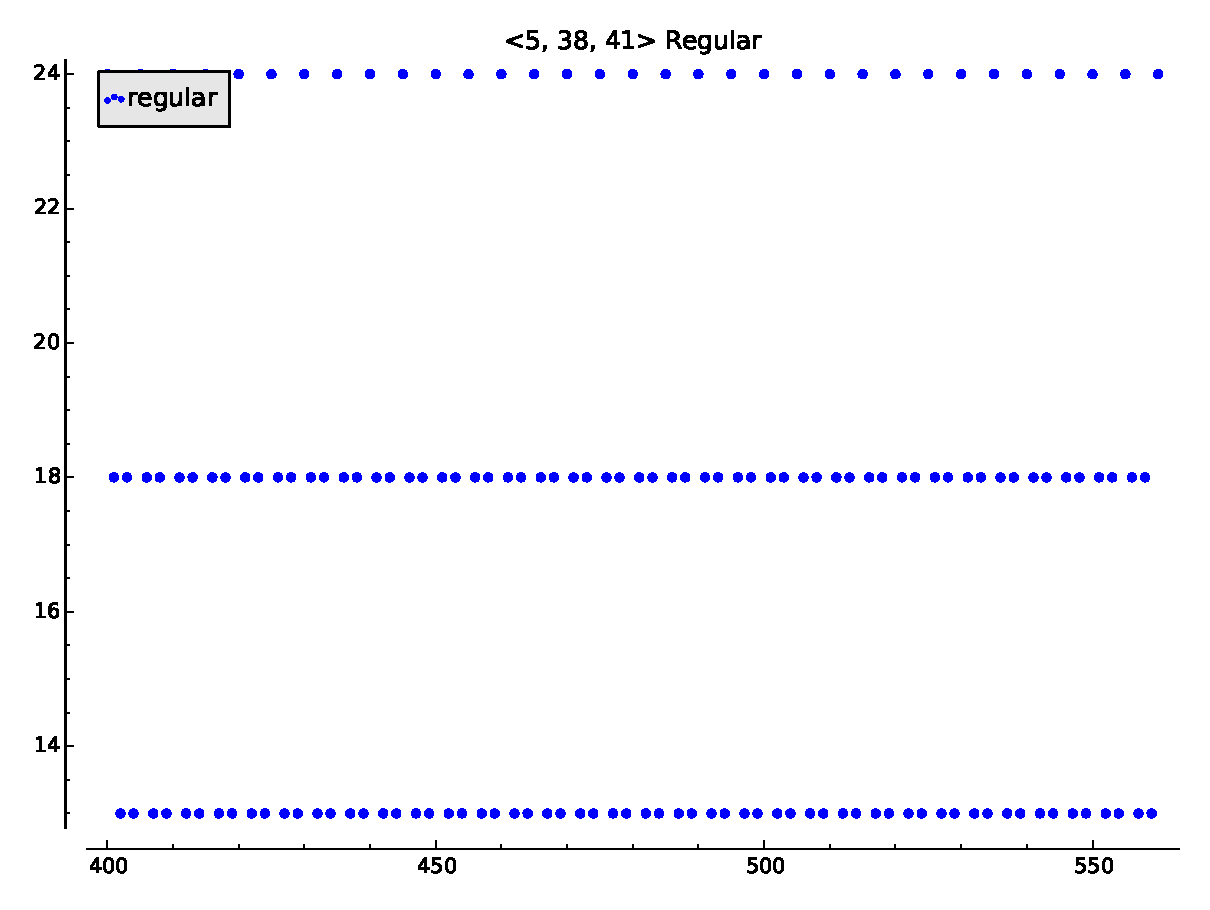
\includegraphics[height = 5.3cm, width=6.45cm]{5-7-3(1).eps}
	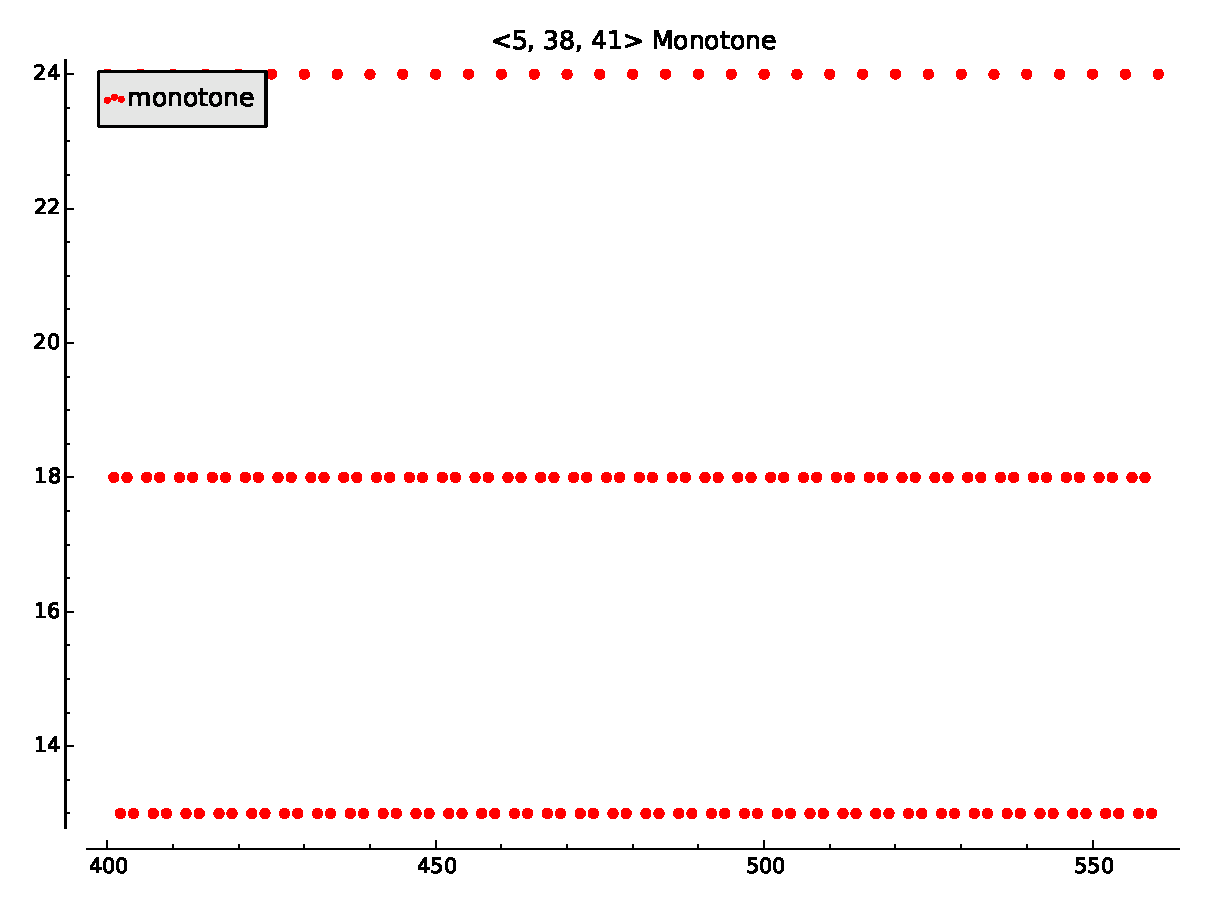
\includegraphics[height = 5.3cm, width=6.45cm]{5-7-3(2).eps}
	}

	\begin{itemize}
	\pause
		\item $c(m) = c_{mon}(m)$\\
	\pause
		\item $c(M) = c_{mon}(M)$
	\end{itemize}
}

\frame{\frametitle{Generalized Arithmetic Sequences}
	\centerline{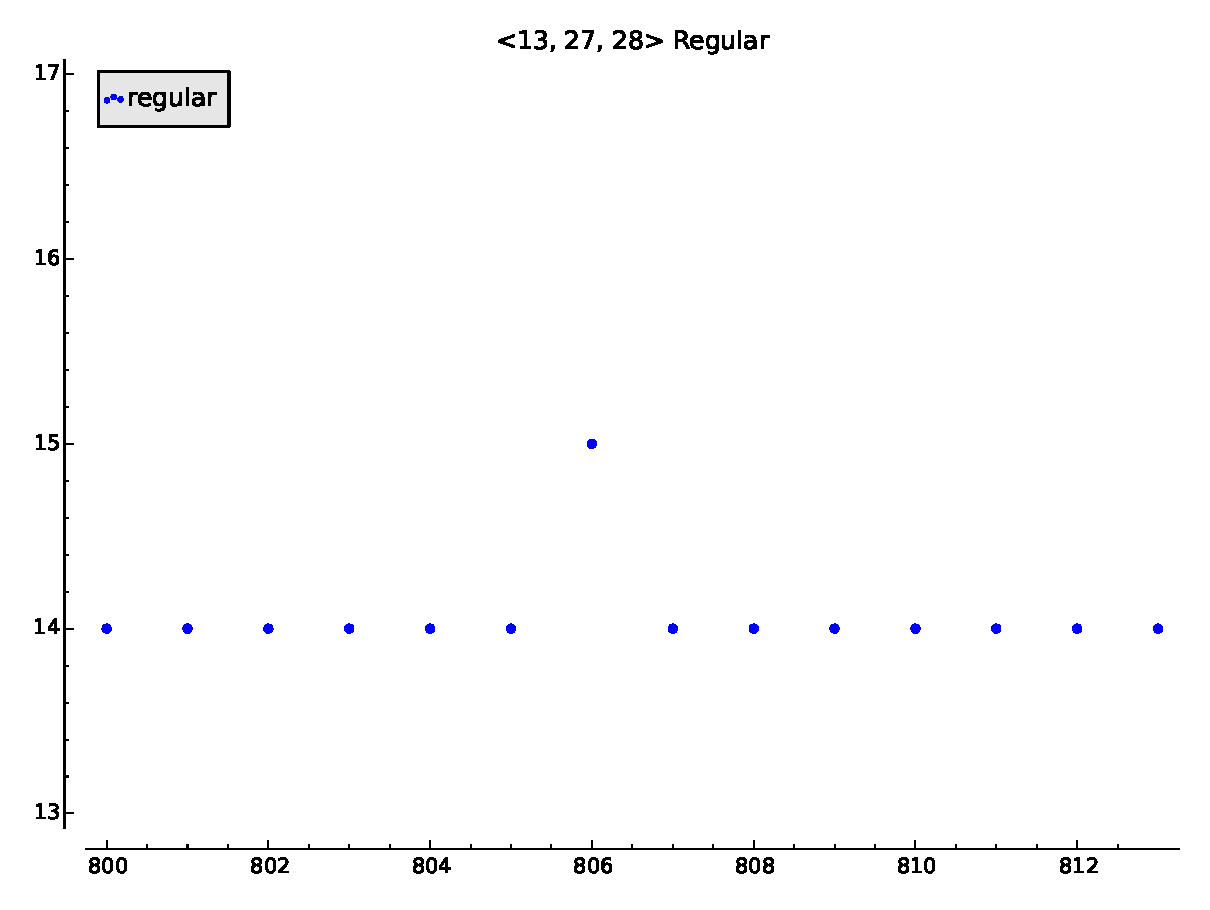
\includegraphics[height = 5.3cm, width=6.45cm]{13-2-1(1).eps}
	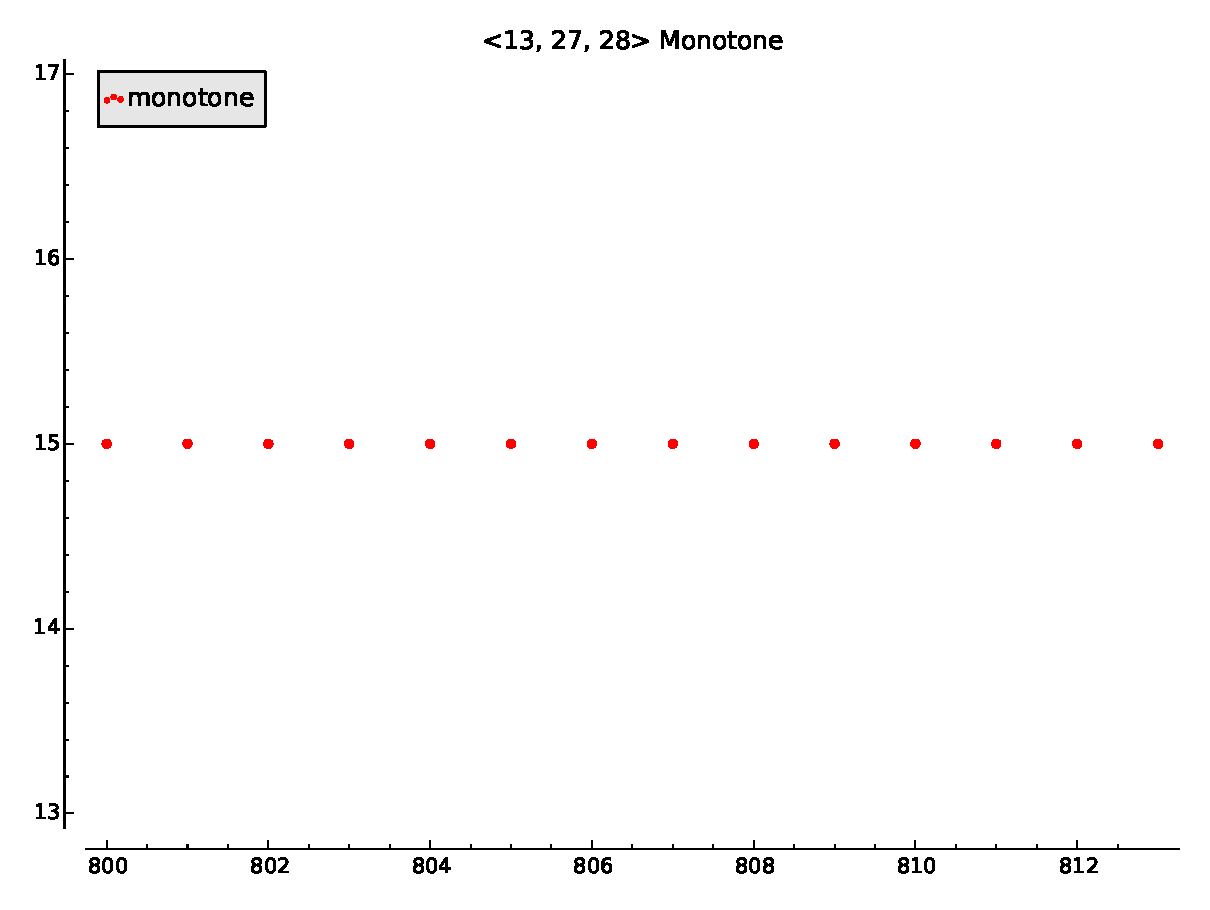
\includegraphics[height = 5.3cm, width=6.45cm]{13-2-1(2).eps}
	}

	\begin{itemize}
	\pause
		\item $c(m) \neq c_{mon}(m)$\\
	\pause
		\item $c(M) = c_{mon}(M)$
	\end{itemize}
}

\frame{\frametitle{Generalized Arithmetic Sequences}
	\centerline{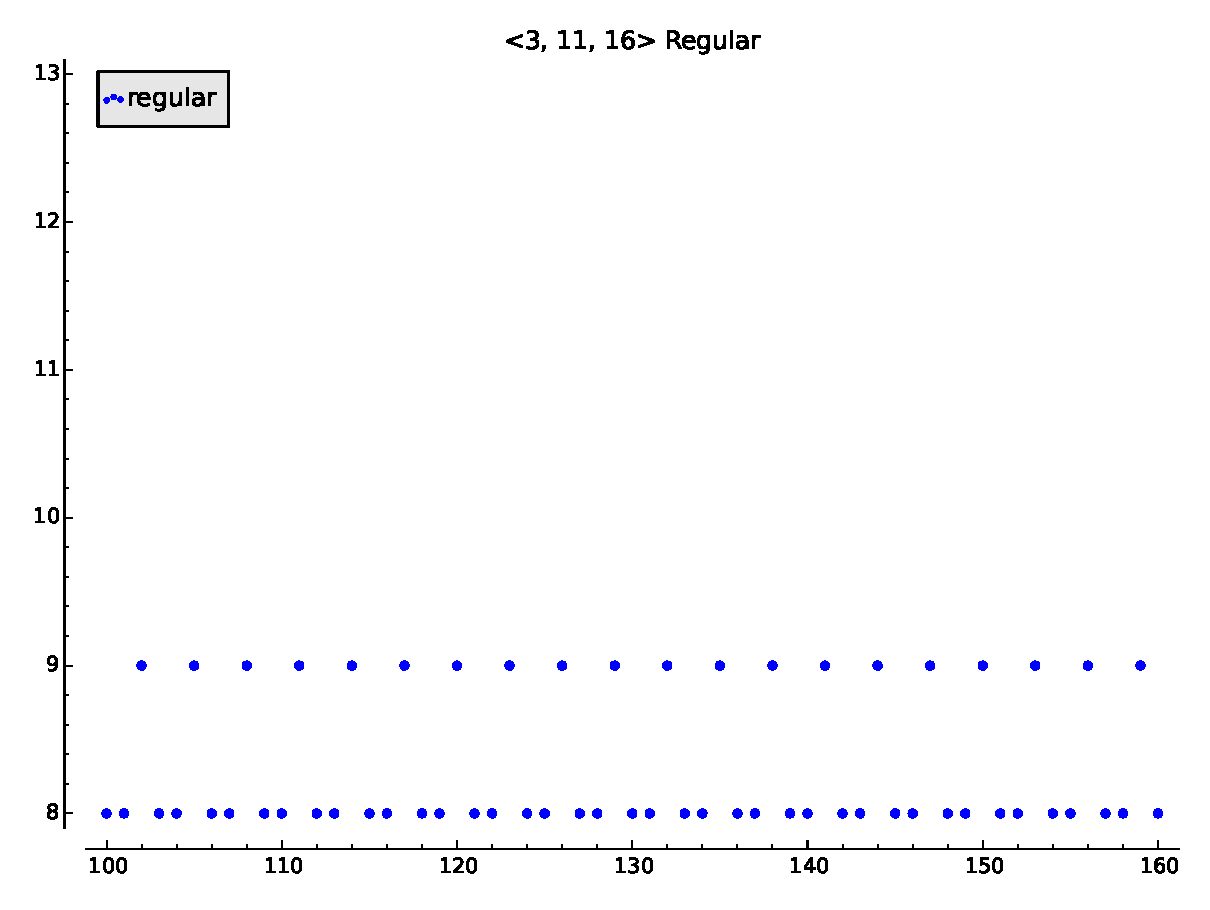
\includegraphics[height = 5.3cm, width=6.45cm]{3-2-5(1).eps}
	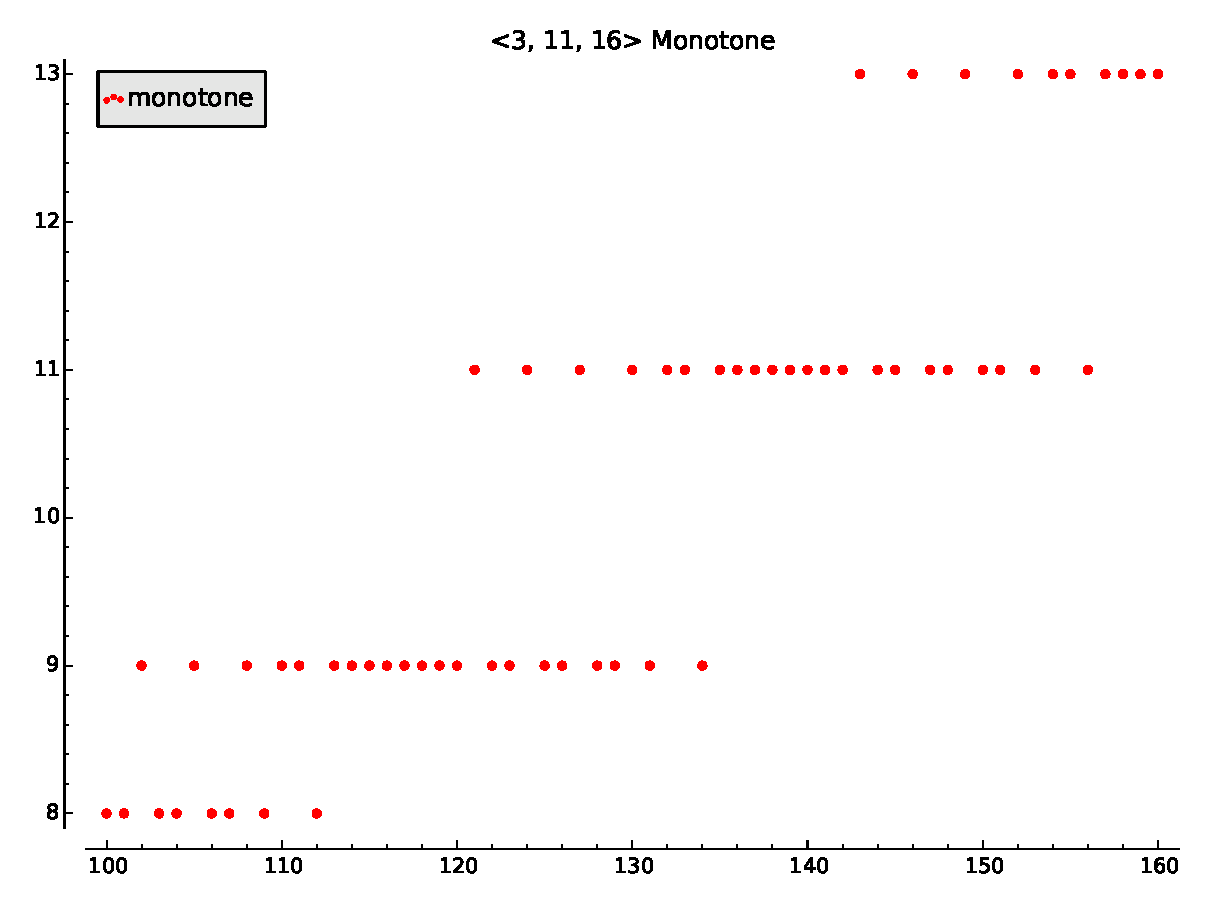
\includegraphics[height = 5.3cm, width=6.45cm]{3-2-5(2).eps}
	}

	\begin{itemize}
	\pause
		\item $c(m) \neq c_{mon}(m)$\\
	\pause
		\item $c(M) < c_{mon}(M)$
	\end{itemize}
}

\frame{\frametitle{Generalized Arithmetic Sequences}
	\begin{conjecture}
		$If \gcd(h - 1, d) > 1$, then $c_{mon}(M) = c(M)$.
	\end{conjecture}
	\pause
	\begin{conjecture}
		$If \gcd(h - 1, d) = 1$, then there are several cases.
		\begin{align*}
			\uncover<3->{&\textbf{Case 1:\;} h < d &\; c(M) < c_{mon}(M)}\\
			\uncover<4->{&\textbf{Case 2:\;} h \geq d \text{ and } c(M) < c_{eq}(M) &\; c(M) < c_{mon}(M)}\\
			\uncover<5>{&\textbf{Case 3:\;} h \geq d \text{ and } c(M) = c_{eq}(M) &\; c(M) = c_{mon}(M)}
		\end{align*}
	\end{conjecture}
}

\frame{\frametitle{Generalized Arithmetic Sequences}
	\begin{minipage}{1.0\textwidth}
	\xymatrix{{} & {} & {} \\
							{\bullet \ar@{.}[u]} & {} & {\bullet \ar@{.}[u]} \\
								{} & {\bullet \ar@{.}[d]} \\
							{} & {} & {}
	}
	\end{minipage}%
	\begin{minipage}{1.0\textwidth}
	\begin{itemize}
		\item \small Recall that $c_{mon}(m) = \max\{c_{eq}(m), c_{adj}(m)\}.$
		\phantom{\parbox{\linewidth}{
		\item $c_{eq}(M) = \frac{ah + 2d - a}{\gcd(h - 1, d)}$
		\item if $\gcd(h - 1, d) > 1$, then $c_{eq}(m) < c_{adj}(m)$
		\item if $\gcd(h - 1, d) = 1$, then $c_{eq}(m) \geq c_{adj}(m)$
		}}
	\end{itemize}
	\end{minipage}
}

\frame{\frametitle{Generalized Arithmetic Sequences}
	\begin{minipage}{1.0\textwidth}
		\xymatrix{{} & {} & {} \\
								{\bullet \ar@{.}[u] \ar@{-}[dr]_{d_1}} & {} & {\bullet \ar@{.}[u] \ar@{-}[dl]^{d_2}} \\
									{} & {\bullet \ar@{.}[d]} \\
								{} & {} & {}
	}
	\end{minipage}%
	\begin{minipage}{1.0\textwidth}
	\begin{itemize}
		\item \small Recall that $c_{mon}(m) = \max\{c_{eq}(m), c_{adj}(m)\}.$
		\phantom{\parbox{\linewidth}{
		\item $c_{eq}(M) = \frac{ah + 2d - a}{\gcd(h - 1, d)}$
		\item if $\gcd(h - 1, d) = 1$, then $c_{eq}(m) \geq c_{adj}(m)$
		\item if $\gcd(h - 1, d) > 1$, then $c_{eq}(m) < c_{adj}(m)$
		}}
	\end{itemize}
	\end{minipage}
}

\frame{\frametitle{Generalized Arithmetic Sequences}
	\begin{minipage}{1.0\textwidth}
	\xymatrix{{} & {} & {} \\
							{\bullet \ar@{.}[u] \ar@{-}[dr]_{d_1} \ar@{-}[rr]^{c_{eq}(m)}} & {} & {\bullet \ar@{.}[u] \ar@{-}[dl]^{d_2}} \\
								{} & {\bullet \ar@{.}[d]} \\
							{} & {} & {}
	}
	\end{minipage}%
	\begin{minipage}{1.0\textwidth}
	\begin{itemize}
		\item \small Recall that $c_{mon}(m) = \max\{c_{eq}(m), c_{adj}(m)\}.$
		\item $c_{eq}(M) = \frac{ah + 2d - a}{\gcd(h - 1, d)}$
		\phantom{\parbox{\linewidth}{
		\item if $\gcd(h - 1, d) = 1$, then $c_{eq}(m) \geq c_{adj}(m)$
		\item if $\gcd(h - 1, d) > 1$, then $c_{eq}(m) < c_{adj}(m)$
		}}
	\end{itemize}
	\end{minipage}
}

\frame{\frametitle{Generalized Arithmetic Sequences}
	\begin{minipage}{1.0\textwidth}
	\xymatrix{{} & {} & {} \\
							{\bullet \ar@{.}[u] \ar@{-}[dr]_{d_1} \ar@{.}[rr]^{c_{eq}(m)}} & {} & {\bullet \ar@{.}[u] \ar@{-}[dl]^{d_2}} \\
								{} & {\bullet \ar@{.}[d]} \\
							{} & {} & {}
	}
	\end{minipage}%
	\begin{minipage}{1.0\textwidth}
	\begin{itemize}
		\item \small Recall that $c_{mon}(m) = \max\{c_{eq}(m), c_{adj}(m)\}.$
		\item $c_{eq}(M) = \frac{ah + 2d - a}{\gcd(h - 1, d)}$
		\item if $\gcd(h - 1, d) = 1$, then $c_{eq}(m) \geq c_{adj}(m)$
		\phantom{\parbox{\linewidth}{
		\item if $\gcd(h - 1, d) > 1$, then $c_{eq}(m) < c_{adj}(m)$
		}}
	\end{itemize}
	\end{minipage}
}

\frame{\frametitle{Generalized Arithmetic Sequences}
	\begin{minipage}{1.0\textwidth}
	\xymatrix{{} & {} & {} \\
							{\bullet \ar@{.}[u] \ar@{-}[dr]_{d_1} \ar@{-}[rr]^{c_{eq}(m)}} & {} & {\bullet \ar@{.}[u] \ar@{-}[dl]^{d_2}} \\
								{} & {\bullet \ar@{.}[d]} \\
							{} & {} & {}
	}
	\end{minipage}%
	\begin{minipage}{1.0\textwidth}
	\begin{itemize}
		\item \small Recall that $c_{mon}(m) = \max\{c_{eq}(m), c_{adj}(m)\}.$
		\item $c_{eq}(M) = \frac{ah + 2d - a}{\gcd(h - 1, d)}$
		\item if $\gcd(h - 1, d) = 1$, then $c_{eq}(m) \geq c_{adj}(m)$
		\item if $\gcd(h - 1, d) > 1$, then $c_{eq}(m) < c_{adj}(m)$
	\end{itemize}
	\end{minipage}
}


%%%%%%%%%%%%%%%%%%%%%%%%%%%%%%%%%%%%
\section[$c_{mon}(M)>c(M)$]{$c_{mon}(M)>c(M)$}

\frame{\frametitle{\texttt{\color{red}{ }}Recall that $c_{mon}(M) \geq c(M)$.}  
\pause When is $c_{mon}(M)>c(M)$? \\ \bigskip \pause
If we have
\begin{itemize}
\item $c_{eq}(M)>c_{adj}(M)$ \pause
\item Whenever $|z_1|=|z_2|=l$ we can find $|z_3| < l$ such that $d(z_1,z_3)<c_{eq}(M)$ and $d(z_2,z_3)<c_{eq}(M)$
\end{itemize} \pause
Then $c_{mon}(M)>c(M)$.
}

\frame{\frametitle{\texttt{\color{red}{ }}Is $c_{mon}(M)>c(M)$?}  
\begin{minipage}[t]{0.48\linewidth}
 \xymatrix{ {\bullet} \\ {\bullet} & {\bullet} \\ {\bullet}  & {\bullet}  & {\bullet}  & {\bullet} \\ {\bullet}  & {\bullet} & {\bullet}  \\ {\bullet} & {\bullet} \\ {\bullet} 
 }

  \end{minipage}
  \begin{minipage}[t]{0.48\linewidth}
   \end{minipage}
  
}

\frame{\frametitle{\texttt{\color{red}{ }}Is $c_{mon}(M)>c(M)$?}  
 \begin{minipage}[t]{0.48\linewidth}
 \xymatrix{ {\bullet} \ar@{-}[dr]\\ {\bullet} & {\bullet}\ar@{-}[d] \\ {\bullet}  & {\bullet}  & {\bullet}\ar@{-}[d]  & {\bullet} \\ {\bullet}\ar@{-}[d]  & {\bullet} & {\bullet}  \\ {\bullet} \ar@{-}[d]& {\bullet} \\ {\bullet} 
 }
 \end{minipage}
  \hfill
  \begin{minipage}[t]{0.48\linewidth}
 \begin{itemize}
  \item $c_{mon}(M)=c_{eq}(M)$. 
  \item Under our restrictions, $c_{eq}(M)>c_{adj}(M)$
   \end{itemize}
\end{minipage}
}
\frame{\frametitle{\texttt{\color{red}{ }}Is $c_{mon}(M)>c(M)$?}  
\begin{minipage}[t]{0.48\linewidth}
 \xymatrix{ {\bullet} \ar@{-}[dr]\\ {\bullet}\ar@{-}[dr] & {\bullet}\ar@{-}[d] \\ {\bullet}\ar@{-}[d]  & {\bullet}\ar@{-}[dl]  & {\bullet}\ar@{-}[d]  & {\bullet}\ar@{-}[dl] \\ {\bullet}\ar@{-}[d]  & {\bullet}\ar@{-}[dl]\ar@{-}[d] & {\bullet}\ar@{-}[dl]  \\ {\bullet} \ar@{-}[d]& {\bullet}\ar@{-}[dl] \\ {\bullet} 
 }
 \end{minipage}
 \hfill
 \begin{minipage}[t]{0.48\linewidth}
  \begin{itemize}
  \item $c_{mon}(M)=c_{eq}(M)$
  \item Under our restrictions, $c_{eq}(M)>c_{adj}(M)$
  \item We can move from two factorizations of length $l$ to one of a lower length with $d<c_{eq}(M)$ \pause 
  \item $c_{mon}(M)>c(M)$
  \end{itemize}
 \end{minipage}
}
%%%%%%%%%%%%%%%%%%%%%%%%%%%%%%%%%%%%
\section[Embedding Dimension Three]{Embedding Dimension Three}

\frame{\frametitle{\texttt{\color{red}{ }}Equivalent Catenary Degree in $\langle 8,9,19 \rangle$}  

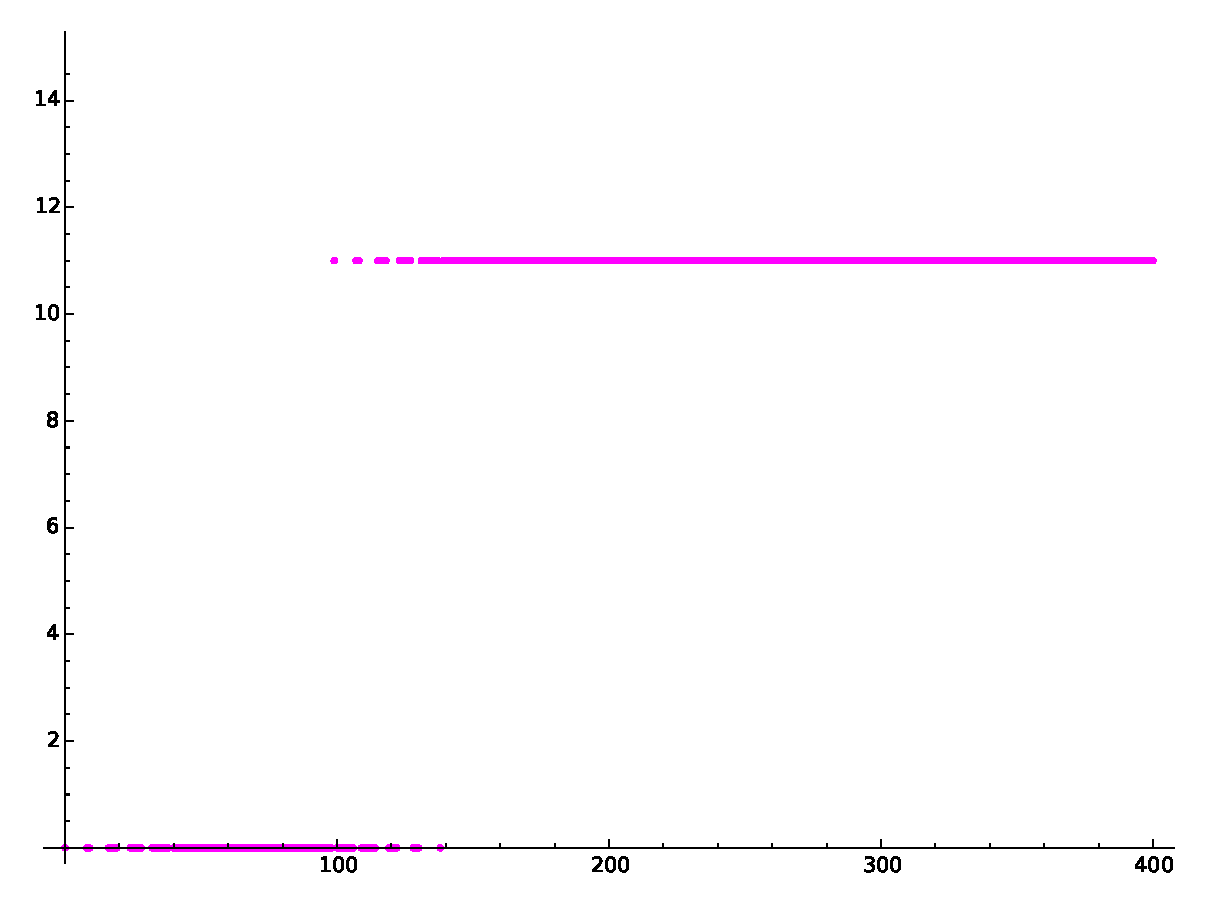
\includegraphics[width=10cm]{equal.eps}

}
\frame{\frametitle{\texttt{\color{red}{ }}Equivalent Catenary Degree in $\langle 8,9,19 \rangle$}  

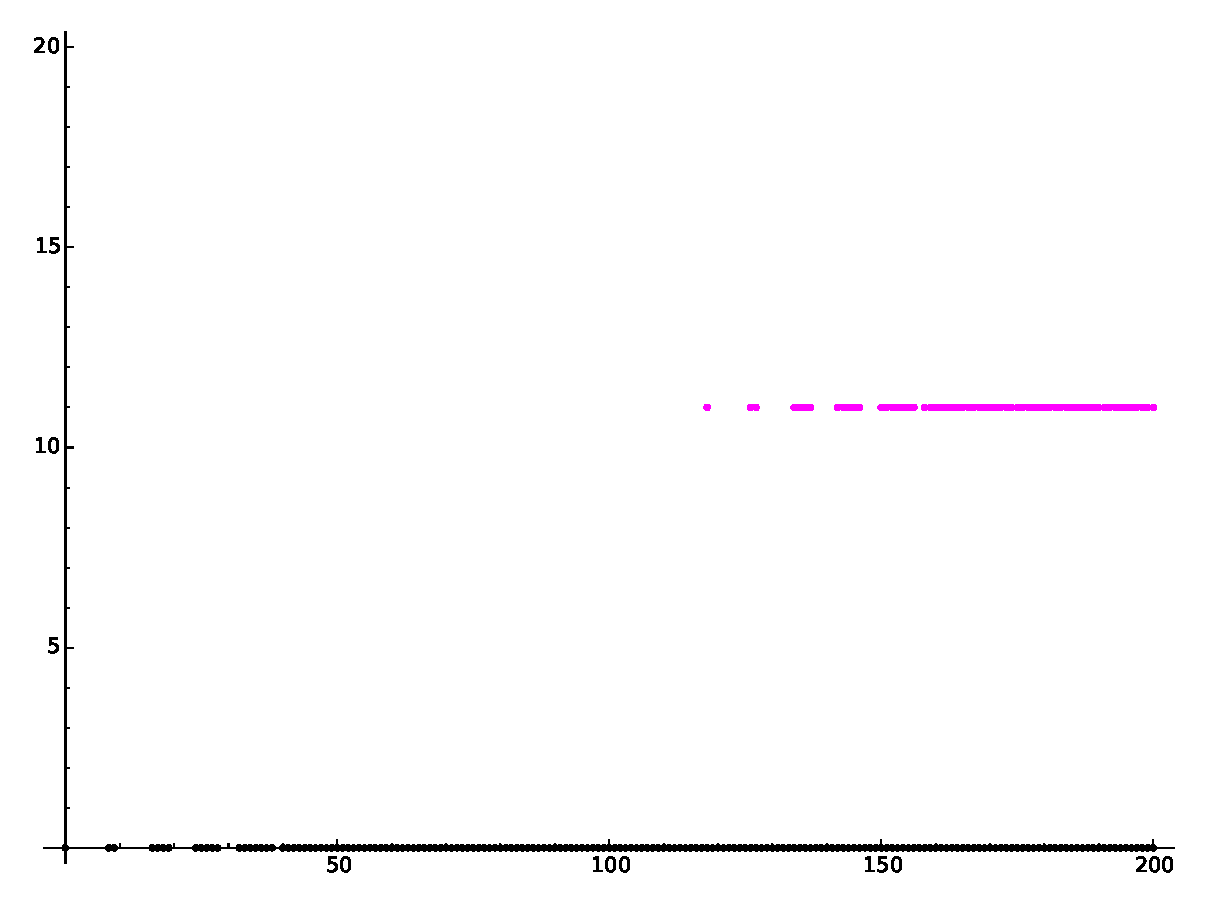
\includegraphics[width=10cm]{equivalent.eps}

}


\frame{\frametitle{\texttt{\color{red}{ }}Equivalent Catenary Degree in $\langle n_1,n_2,n_3 \rangle$}  
\begin{theorem}
Let $M$ be a minimally generated numerical monoid $\langle n_1,n_2,n_3 \rangle$. Then $c_{eq}(M)=\frac{n_3-n_1}{gcd(n_2-n_1,n_3-n_1)}$
\end{theorem} \pause
\begin{itemize}
\item If $m=n_2\left(\frac{n_3-n_1}{gcd(n_2-n_1,n_3-n_1)}\right)+x$ for some $x \in M$, then $c_{eq}(m)=c_{eq}(M)$.
\item If $m=n_2\left(\frac{n_3-n_1}{gcd(n_2-n_1,n_3-n_1)}\right)+x$ for some $x \notin M$, then $c_{eq}(m)=0$.

\end{itemize}

}
\frame{\frametitle{\texttt{\color{red}{ }}Equivalent Catenary Degree in $\langle n_1,n_2,n_3 \rangle$}  
\begin{theorem}
For all $m \in M$ such that $m>n_2\left(\frac{n_3-n_1}{gcd(n_2-n_1,n_3-n_1)}\right)+\mathcal{F}(M)$, $c_{eq}(m)=c_{eq}(M)$. Furthermore, $c_{eq}(m)$ can take on only two values: $0$ and $c_{eq}(M)$.
\end{theorem} 

}
\frame{\frametitle{\texttt{\color{red}{ }}Moving Between Factorizations}  
$$M= \langle n_1, n_2, n_3 \rangle $$
To calculate $c_{eq}$ we needed a way to move between factorizations of the same length. \pause \\ \medskip
Let $z_1=(b,c,d)$ and let $|z_1|=|z_2|$. Then $$z_2=\left(b+\frac{k(n_3-n_1)}{n_3-n_1}-k,c-\frac{k(n_3-n_1)}{n_3-n_1},d+k\right)$$
\\ \bigskip
\pause
What if we want to move between factorization lengths?  \pause
\begin{theorem}
Consider a factorization $z=(b,c,d)$ of an element $s \in M$ with $|z|=x$. We can write any factorization $z_i$ of $s$ where $|z_i|=x\textcolor{red}{-l}$ as $z_i=\left(b+\frac{\textcolor{red}{-ln_1}+k(n_3-n_1)}{n_3-n_1}-k\textcolor{red}{-l},c+\frac{\textcolor{red}{ln_1}-k(n_3-n_1)}{n_3-n_1},d+k\right)$.
\end{theorem}
}
%%%%%%%%%%%%%%%%%%%%%%%%%%%%%%%%%%%%

%%%%%%%%%%%%%%%%%%%%%%%%%%%%%%%%%%%%

\frame{\frametitle{When is $c_{mon}(M)>c(M)$?}	
	For certain families of monoids, we can guarantee that our two conditions for $c_{mon}(M)>c(M)$ hold. \pause \bigskip \\
	$M=\langle  na,na+n,2na+nx+1 \rangle $ with $x \geq 2$ \\ \bigskip \pause
	Recall that $c_{mon}(M) = \max\{c_{eq}(M),c_{adj}(M)\}$. \\ \bigskip \pause
	\begin{itemize}
	\item $c_{eq}(M)=na+nx+1$ \\ \medskip \pause
	\item $c_{adj}(M) < na+nx+1$ 
	\end{itemize}
}
\frame{\frametitle{$\langle na,na+n,2na+nx+1 \rangle $}	
	
	$M=\langle na,na+n,2na+nx+1 \rangle $ with $x \geq 2$ \\ \bigskip

 \pause 
 \xymatrix{ {\bullet}z_1 \ar@{-}[d]_{nx+1} & {\bullet}z_2 \ar@{-}[dl]^{na+n} \\ {\bullet}z_3
 } \pause
\begin{theorem}
Let $M=\langle na,na+n,2na+nx+1 \rangle $ for $n \in \mathbb{N}$ and $x \geq 2$. Then $c_{mon}(M)>c(M)$.
\end{theorem}
		
}



\frame{\frametitle{\texttt{\color{red}{ }}$\langle a,a+1,\mathcal{F} \langle a,a+1 \rangle \rangle$}
We have shown that in many cases, $c_{mon}(M)>c(M)$. \\ \medskip
\pause
How big can the difference be between $c_{mon}(M)$ and $c(M)$? \pause
$$\langle a, a+1,\mathcal{F} \langle a,a+1 \rangle \rangle$$
\begin{itemize}
\item $c_{mon}(M)=a^2-2a-1$
\item $c(M)=2a-3$ \pause
\item $c_{mon}(M)-c(M)=a^2-4a-4$
\end{itemize}
}


\frame{\frametitle{\texttt{\color{red}{ }}$\langle a,a+1,\mathcal{F} \langle a,a+1 \rangle \rangle$}
\includegraphics[width=10cm]{plot.eps}
}

\frame{\frametitle{\texttt{\color{red}{ }}$c_{mon}(M)-c(M)$}
\begin{theorem}
	The difference between the monotone and regular catenary degrees of a monoid can be arbitrarily large. 
	\end{theorem}	
	}
\frame{\frametitle{\texttt{\color{red}{ }}Takeaways}
	\begin{itemize}
	\item In some monoids, namely those generated by arithmetic sequences, $c_{mon}(M)=c(M)$. 
	\pause
	\item In generalized arithmetic monoids, we can have either $c_{mon}(M)>c(M)$ or $c_{mon}(M)=c(M)$. 
	\pause
	\item In general, we expect that $c_{mon}(M)>c(M)$. In fact, the difference between the two can grow arbitrarily large. 
	\end{itemize}
}


%%%%%%%%%%%%%%%%%%%%%%%%%%%%%%%%%%%%
\section{Acknowledgements} 

\frame{\frametitle{\texttt{\color{red}{ }}Thank You}  
We would like to thank:
\begin{itemize}
\item The NSF and NSA
\item Sam Houston State University, University of Hawai'i at Hilo, and PURE Math
\item Dr. Brian Loft, Dr. Rebecca Garc\'ia, and Dr. Luis Garc\'ia
\item Dr. Brian Wissman, Dr. Bob Pelayo
\item Dr. Scott Chapman and Dr. Chris O'Neill
\item Felix Gotti and Marly Cormar
\end{itemize}
}

\section[References]{References}

\frame{\frametitle{\texttt{\color{red}{ }}References}  

\begin{itemize}

	\item Bowles, Craig, Scott T. Chapman, Nathan Kaplan, and Daniel Reiser. "On Delta Sets Of Numerical Monoids." \textit{Journal of Algebra and Its Applications J. Algebra Appl.} \textbf{05} (2006), 695-718. \\

	\item S. T. Chapman, M. Corrales, A. Miller, C. Miller, and D. Patel. \textit{The Catenary Degrees of Elements in Numerical Monoids Generated by Arithmetic Sequences}. Journal of the Australian Mathematical Society, 2014. \\
	
	\item S. T. Chapman, P. A. Garc�a-S�nchez, and D. Llena. "The Catenary and Tame Degree of Numerical Monoids." \textit{Forum Mathematicum} \textbf{21} (2009). \\


	\item A. Geroldinger and P. Yuan, The Monotone Catenary Degree of Krull Monoids, \textit{Results in Mathematics} \textbf{63}(2013), 999-1031. \\
	
\end{itemize}	
}	

\frame{\frametitle{References}
	
\begin{itemize}

	\item M. Omidali. "The Catenary and Tame Degree of Numerical Monoids Generated by Generalized Arithmetic Sequences." \textit{Forum Mathematicum}. \textbf{24} (2012), 627-640.

	\item A. Philip, A characterization of arithmetical invariants by the monoid of relations II: The monotone catenary degree and applications to semigroup rings, \textit{Semigroup Forum} \textbf{81} (2010), 424-434. \\
	
	\item J. C. Rosales and P. A. Garc\'ia-S\'anchez, \textit{Finitely generated commutative monoids}, Nova Science Publishers, NewYork, 1999.
	
\end{itemize}	
}







\end{document}